\section{Översikt av system}
På plattformen kommer tre moduler att installeras:

\begin{itemize}
\item Huvudmodul
\item Styrmodul
\item Sensormodul
\end{itemize}
\subsection{Kommunikation}
Kommunikationen mellan Huvudmodulen, styrmodulen och sensormodulen kommer att ske över UART. Huvudmodulen kommer ha två stycken USB-RS232 konverterare som kommer kopplas till var sin modul. Kommunikationen från Beagleboard till PC kommer att ske över USB. Förslaget är att sätta upp ett PAN (PERSONAL AREA NETWORK) mellan PC:n och BB över bluetooth. Detta möjligör kommunikation över TCP/IP protokollet.
\newline
\centerline{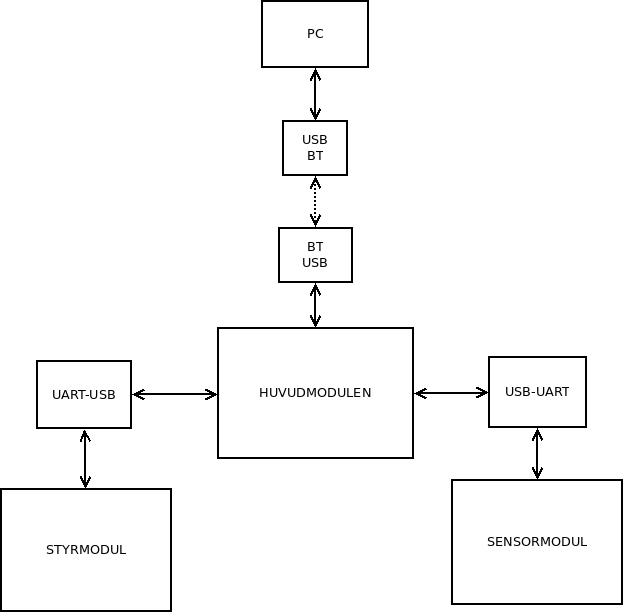
\includegraphics[scale=0.4]{FLOW1PNG}}
